\documentclass[aspectratio=169, 10pt]{beamer}

%  Theme & Colors 
\usetheme{Madrid}
\usecolortheme{whale}
\definecolor{dtblue}{RGB}{180,0,0}
\definecolor{dtgreen}{RGB}{180,0,0}
\definecolor{dtorange}{RGB}{80,0,0}
\setbeamercolor{palette primary}{bg=black,fg=white}
\setbeamercolor{palette secondary}{bg=black!85,fg=white}
\setbeamercolor{palette tertiary}{bg=black,fg=white}
\setbeamercolor{palette quaternary}{bg=black,fg=white}
\setbeamercolor{structure}{fg=black}
\setbeamercolor{title}{fg=white,bg=black}
\setbeamercolor{frametitle}{fg=white,bg=black}
\setbeamercolor{block title}{bg=black,fg=white}
\setbeamercolor{block body}{bg=black!5}
\setbeamercolor{block title alerted}{bg={rgb:red,180;green,0;blue,0},fg=white}
\setbeamercolor{block body alerted}{bg=red!5}
\setbeamercolor{block title example}{bg=black!75,fg=white}
\setbeamercolor{block body example}{bg=black!5}
\setbeamercolor{itemize item}{fg={rgb:red,180;green,0;blue,0}}
\setbeamercolor{itemize subitem}{fg=black}
\setbeamercolor{footline}{bg=black,fg=white}
\setbeamercolor{navigation symbols}{fg=black}

\usepackage{booktabs}
\usepackage{graphicx}
\usepackage{fontawesome5}
\usepackage{tikz}
\usetikzlibrary{shapes.geometric, arrows.meta, positioning, calc}
\usepackage{pgfpages}
\setbeameroption{show notes on second screen=right}
\setbeamertemplate{note page}{\pagecolor{yellow!8}\insertnote}

%  Metadata 
\title[DT Health Pathology]{Digital Twin for AI-Enhanced Pathology Report\\Analysis \& Cross-Referencing}
\subtitle{State of the Art, Our Differentiation \& Hypothesis}
\author{DT Health Pathology Team}
\date{April 2026}
\institute{}

\begin{document}

% =====================================================================
% SLIDE 0 — Catchy Intro
% =====================================================================
{\setbeamercolor{background canvas}{bg=black}
\begin{frame}[plain]
\vfill
\begin{center}
{\color{white}\Huge\bfseries What if AI could read\\[6pt]
\textcolor{dtblue}{every pathology report}\\[6pt]
and support medical decisions and prognosis?}
\vspace{18pt}

{\color{white!70}\large From pathology reports to structured clinical insight\\[4pt]
at scale.}
\vspace{24pt}

{\color{white!50}\normalsize April 2026}
\end{center}
\vfill
\end{frame}
}
\note{
\begin{itemize}
\item Imagine processing every pathology report a hospital has ever generated.
\item We build a DT that reads, extracts, and cross-references at massive scale.
\item AI does not replace clinical rules  it enhances data analysis.
\end{itemize}
}

% =====================================================================
% SLIDE 1 — State-of-the-Art: Top Nature & High-Impact Papers
% =====================================================================
\begin{frame}{State of the Art: Latest High-Impact Papers}

\begin{columns}[T]
\begin{column}{0.48\textwidth}

\begin{block}{\faFile\ \ Top Papers (2024--2026)}
\footnotesize
\begin{enumerate}\setlength{\itemsep}{3pt}
    \item \textbf{Eminaga et al.} (2024) \textit{Sci.\ Reports} (Nature)\\
    \textcolor{dtblue}{``Critical Evaluation of AI as a Digital Twin of Pathologists for Prostate Cancer Pathology''} : vPatho system
    \item \textbf{Marchal} (2025) \textit{Nat.\ Biotechnology}\\
    \textcolor{dtblue}{``Applications of Digital Twins in Medicine''} : Perspective on DT frameworks
    \item \textbf{G\"ortz et al.} (2026) \textit{Nat.\ Rev.\ Urology}\\
    \textcolor{dtblue}{``Digital Twins for Personalized Treatment in Uro-Oncology in the Era of AI''} : Review
\end{enumerate}
\end{block}

\end{column}

\begin{column}{0.50\textwidth}

\begin{alertblock}{\faLightbulb\ \ Their Novelty}
\footnotesize
\begin{itemize}\setlength{\itemsep}{2pt}
    \item[\faCheckCircle] \textbf{vPatho:} First systematic benchmark of AI as a ``digital twin'' of a pathologist; compared with 6 human experts on Gleason grading
    \item[\faCheckCircle] \textbf{Marchal:} Conceptual framework for bidirectional patient--model data flow in clinical DTs
    \item[\faCheckCircle] \textbf{G\"ortz:} Comprehensive DT roadmap for uro-oncology integrating imaging, genomics \& treatment simulation
\end{itemize}
\end{alertblock}

\begin{exampleblock}{\faTimes\ \ Their Limitations}
\footnotesize
\begin{itemize}\setlength{\itemsep}{2pt}
    \item Single cancer type (prostate) focus
    \item Image-only analysis : no NLP (No expert feedback) on pathology \textit{reports}
    \item No cross-referencing against AJCC knowledge base
    \item No automated data discovery or crawling pipeline
\end{itemize}
\end{exampleblock}

\end{column}
\end{columns}

\end{frame}
\note{
\begin{itemize}
\item Most AI pathology systems operate in isolation from clinical standards.
\item Eminaga (vPatho): first AI-vs-pathologist benchmark on Gleason grading.
\item Marchal: bidirectional patient--model data flow framework.
\item G\"ortz: DT roadmap for uro-oncology with imaging and genomics.
\item Common gap: image-only, single cancer, no NLP on reports, no AJCC.
\item We propose a clinically grounded DT that processes reports at scale.
\end{itemize}
}

% =====================================================================
% SLIDE 2 — Our Differentiation
% =====================================================================
\begin{frame}{How We Differ: Our DT Health Pathology Approach}

\begin{columns}[T]
\begin{column}{0.48\textwidth}

\begin{block}{\faList\ \ Key Differentiators}
\footnotesize
\begin{tabular}{@{}p{1.8cm}p{1.6cm}p{2.2cm}@{}}
\toprule
\textbf{Feature} & \textbf{State of Art} & \textbf{Our Approach} \\
\midrule
Data Input & Images only & \textcolor{dtgreen}{\textbf{Reports + Clinical}} \\
Analysis & AI grading & \textcolor{dtgreen}{\textbf{Cross-Ref AJCC KB}} \\
Staging & AI predicts & \textcolor{dtgreen}{\textbf{Rule-based (fixed)}} \\
Cancer Scope & Single type & \textcolor{dtgreen}{\textbf{Multi-cancer}} \\
Data Discovery & Static & \textcolor{dtgreen}{\textbf{MCP Crawl Agent}} \\
Human Loop & None & \textcolor{dtgreen}{\textbf{mRAG HILF}} \\
LLM Stack & N/A & \textcolor{dtgreen}{\textbf{KG}} \\
\bottomrule
\end{tabular}
\end{block}

\end{column}

\begin{column}{0.50\textwidth}

\begin{exampleblock}{\faRocket\ \ Disruptive Outcomes}
\footnotesize
\begin{itemize}\setlength{\itemsep}{2pt}
    \item NLP-first Digital Twin for pathology \textit{text} reports
    \item Staging follows \textbf{AJCC fixed rules}  AI \textbf{enhances, extracts \& cross-references} data against the AJCC knowledge base
    \item MCP-powered crawling agent for automated real-time data discovery and ingestion
    \item Scenario-based Knowledge Graph with LLM orchestration
\end{itemize}
\end{exampleblock}

\begin{alertblock}{\faLightbulb\ \ Core Insight}
\footnotesize
\textit{The AI pipeline does \textbf{not replace} rule-based AJCC staging. Instead, LLMs extract structured fields from free-text reports and cross-reference them against the AJCC book, enabling richer analysis and expert validation.}
\end{alertblock}

\end{column}
\end{columns}

\end{frame}
\note{
\begin{itemize}
\item We process free-text reports and clinical records, not images.
\item AJCC staging is deterministic  AI extracts and cross-references, not predicts.
\item MCP crawling agent automates data discovery in real time.
\item Human-in-the-loop via mRAG keeps clinicians in control.
\item System works across multiple cancer types, not just prostate.
\end{itemize}
}

% =====================================================================
% SLIDE 3 — Metrics, Hypothesis & Data
% =====================================================================
\begin{frame}{Metrics, Hypothesis \& Data Architecture}

\begin{columns}[T]
\begin{column}{0.48\textwidth}

\begin{block}{\faFlask\ \ Research Hypothesis}
\tiny
\textit{``A Digital Twin architecture that uses LLMs to extract, harmonize, and cross-reference pathology report data against the AJCC knowledge base  with human-in-the-loop feedback  can \textbf{further analyse multimodal clinical data at scale} and potentially \textbf{support medical prognosis}, enabling richer insight discovery across multiple cancer types by processing massive volumes of pathology reports and clinical records that would be infeasible for manual expert review.''}
\end{block}

\vspace{2pt}
\begin{alertblock}{\faChartBar\ \ Evaluation Metrics}
\scriptsize
\begin{itemize}\setlength{\itemsep}{1pt}
    \item \textbf{Extraction Accuracy:} Precision, Recall, F1 for entity/field extraction from reports
    \item \textbf{Cross-Ref.\ Consistency:} Agreement rate between LLM output and AJCC rule-based staging
    \item \textbf{Inter-rater Agreement:} Cohen's $\kappa$ between DT output and experts
    \item \textbf{Data Quality:} QA/QC pass rate, completeness, provenance
    \item \textbf{Efficiency:} Expert review time reduction (\%), cycles saved
    \item \textbf{Statistical Validation:} Mann--Kendall test, variable importance
\end{itemize}
\end{alertblock}

\end{column}

\begin{column}{0.50\textwidth}

\begin{exampleblock}{\faDatabase\ \ Data Sources \& Pipeline}
\scriptsize
\begin{itemize}\setlength{\itemsep}{1pt}
    \item[{\faBook}] \textbf{AJCC Cancer Staging Manual}  Full book as TNM knowledge base
    \item[{\faFile}] \textbf{Pathology Reports}  Free-text (breast cancer primary, extensible)
    \item[{\faHospital}] \textbf{Clinical Data}  Demographics, treatment, lab results
    \item[{\faRobot}] \textbf{MCP Crawling Agent}  Automated data discovery \& ingestion
    \item[{\faCogs}] \textbf{Data Warehouse}  Harmonized repository + provenance tracking
\end{itemize}
\end{exampleblock}

\vspace{4pt}
\begin{block}{\faLayerGroup\ \ Technology Stack}
\footnotesize
\begin{center}
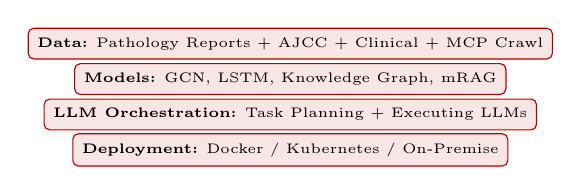
\begin{tikzpicture}[
    every node/.style={font=\tiny, minimum height=0.4cm},
    layer/.style={rounded corners=2pt, draw=dtblue, fill=dtblue!10, 
                  minimum width=5cm, minimum height=0.35cm}
]
\node[layer] (l1) at (0,0) {\textbf{Deployment:} Docker / Kubernetes / On-Premise};
\node[layer] (l2) at (0,0.45) {\textbf{LLM Orchestration:} Task Planning + Executing LLMs};
\node[layer] (l3) at (0,0.9) {\textbf{Models:} GCN, LSTM, Knowledge Graph, mRAG};
\node[layer] (l4) at (0,1.35) {\textbf{Data:} Pathology Reports + AJCC + Clinical + MCP Crawl};
\end{tikzpicture}
\end{center}
\end{block}

\end{column}
\end{columns}

\end{frame}
\note{
\begin{itemize}
\item Hypothesis: LLM-based DT can analyse multimodal data at scale and support prognosis.
\item We use the entire AJCC book as a structured knowledge base.
\item Primary data: free-text pathology reports, starting with breast cancer.
\item Metrics: extraction F1, AJCC cross-ref consistency, Cohen's kappa, QA/QC rates.
\item Efficiency measured by expert review time reduction.
\item Statistical validation via Mann--Kendall and variable importance.
\end{itemize}
}

% =====================================================================
% SLIDE 3b — TCGA / GDC as Validation Dataset & Hypothesis
% =====================================================================
\begin{frame}[fragile]{TCGA via GDC: Open Dataset \& Research Hypothesis}

\begin{columns}[T]
\begin{column}{0.48\textwidth}

\begin{block}{\faDatabase\ \ What TCGA/GDC Provides}
\scriptsize
\begin{itemize}\setlength{\itemsep}{2pt}
    \item \textbf{Pathology Reports:} Free-text surgical/pathology PDFs for 33 cancer types ($\sim$11{,}000 cases)
    \item \textbf{Structured TNM:} AJCC stage, T/N/M fields, histology, grade per case
    \item \textbf{Clinical Outcomes:} Overall survival, disease-free survival, treatment records
    \item \textbf{Multi-omics:} Genomics, proteomics, imaging  extensible for future fusion
    \item \textbf{Open Access:} Programmatic REST API + \texttt{gdc-client} Python library; no credentials for open-tier data
\end{itemize}
\end{block}

\begin{exampleblock}{\faCode\ \ Programmatic Access}
\tiny
\begin{verbatim}
POST https://api.gdc.cancer.gov/files
{
  "filters": {
    "op": "and", "content": [
      {"op":"=","content":{
        "field":"cases.project.project_id",
        "value":"TCGA-BRCA"}},
      {"op":"=","content":{
        "field":"data_type",
        "value":"Pathology Report"}}
    ]
  },
  "fields": "file_id,cases.diagnoses.tumor_stage"
}
\end{verbatim}
\end{exampleblock}

\end{column}

\begin{column}{0.50\textwidth}

\begin{alertblock}{\faFlask\ \ TCGA-Grounded Hypothesis}
\scriptsize
\textit{``By applying the DT Health Pathology NLP pipeline to \textbf{TCGA open-access pathology reports}, we hypothesise that LLM-extracted TNM fields will achieve \textbf{F1 $\geq$ 0.85} against the structured AJCC ground truth labels already present in GDC, and that the resulting cross-referenced knowledge graph will reveal \textbf{statistically significant associations} between report-derived biomarkers and survival outcomes across $\geq$3 cancer types  validating the pipeline at scale before deployment on proprietary institutional data.''}
\end{alertblock}

\vspace{4pt}
\begin{block}{\faCheckCircle\ \ Why TCGA is Ideal for Validation}
\scriptsize
\begin{itemize}\setlength{\itemsep}{2pt}
    \item Ground-truth TNM labels $\rightarrow$ direct F1 / AJCC consistency measurement
    \item Free-text reports + structured outcomes $\rightarrow$ end-to-end prognosis pipeline test
    \item Multi-cancer scope $\rightarrow$ tests generalization before clinical deployment
    \item No PHI barrier for open tier $\rightarrow$ fast iteration and reproducibility
\end{itemize}
\end{block}

\end{column}
\end{columns}

\end{frame}
\note{
\begin{itemize}
\item TCGA/GDC is the ideal open benchmark: free-text reports AND ground-truth TNM labels in the same dataset.
\item We can compute F1 for NLP extraction directly against GDC structured fields.
\item Survival data (OS, DFS) lets us test whether extracted biomarkers are prognostically informative.
\item No credentials needed for open-tier; MCP crawling agent can hit the REST API directly.
\item Starting with TCGA-BRCA (breast) then extending to LUAD, COAD, etc.
\item This slide bridges the hypothesis (Slide 3) to the architecture (Slide 4).
\end{itemize}
}

% =====================================================================
% SLIDE 4 — Architecture Overview (Picture1.pdf)
% =====================================================================
\begin{frame}{Architecture Overview}
\begin{center}
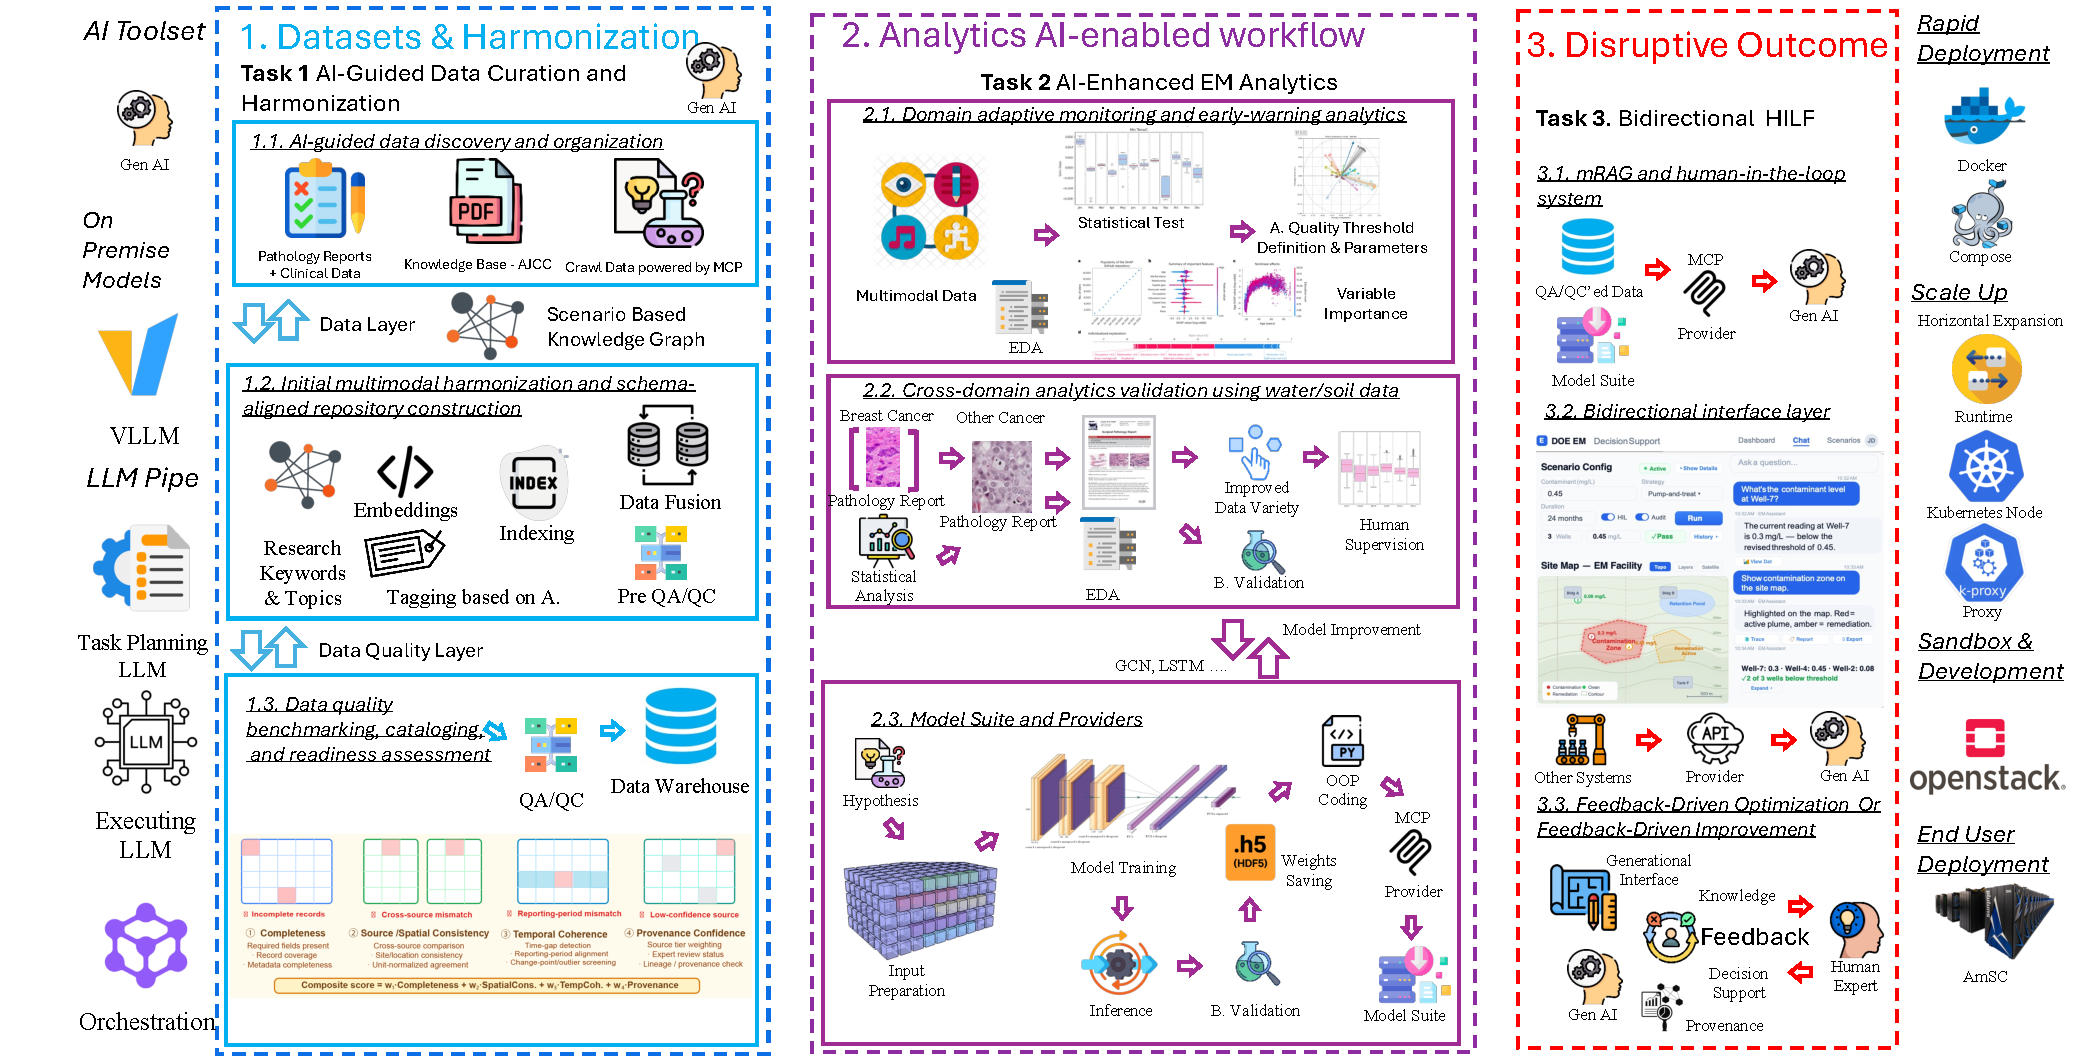
\includegraphics[width=0.92\textwidth, height=0.82\textheight, keepaspectratio]{Picture1.pdf}
\end{center}
\note{
\begin{itemize}
\item Data layer: reports, clinical records, AJCC KB ingested via MCP agent.
\item Model layer: GCN, LSTM, knowledge graph, multimodal RAG.
\item LLM orchestration coordinates task planning and execution.
\item Human-in-the-loop interface for expert review and feedback.
\item Containerised with Docker/Kubernetes, deployable on-premise.
\end{itemize}
}
\end{frame}

% =====================================================================
% SLIDE 5a — Research Goal
% =====================================================================
\begin{frame}{Research Goal}

\begin{columns}[T]
\begin{column}{0.52\textwidth}

\begin{block}{\faBullseye\ \ Goal}
\normalsize
Build a \textbf{Digital Twin (DT)} that ingests free-text clinical pathology reports, extracts structured oncological data using LLMs, and cross-references it against the AJCC Cancer Staging knowledge base  enabling \textbf{automated, scalable prognosis support} across multiple cancer types with human-in-the-loop validation.
\end{block}

\vspace{8pt}
\begin{block}{\faExclamationCircle\ \ Key Constraint}
\small
\textbf{AI does not predict staging.}\\[4pt]
AJCC TNM staging follows deterministic, rule-based criteria. The LLM \textit{extracts} and \textit{cross-references} data  it \textbf{never overrides} clinical rules. 
% This ensures clinical safety and regulatory compliance.
\end{block}

\end{column}

\begin{column}{0.44\textwidth}

\begin{exampleblock}{\faLayerGroup\ \ What the System Does}
\small
\begin{enumerate}\setlength{\itemsep}{6pt}
    \item \textbf{Ingest} free-text pathology reports\\(TCGA/GDC + institutional)
    \item \textbf{Extract} TNM fields, histology \& biomarkers via LLMs
    \item \textbf{Cross-reference} against AJCC fixed staging rules
    \item \textbf{Enrich} with a multi-cancer Knowledge Graph
    \item \textbf{Surface} insights via mRAG + expert feedback loop
\end{enumerate}
\end{exampleblock}

\end{column}
\end{columns}

\end{frame}
\note{
\begin{itemize}
\item The core goal: DT that reads free-text reports and cross-references against AJCC at scale.
\item Key constraint is critical for clinical credibility: AI extracts and cross-references, never predicts staging.
\item AJCC rules are deterministic  LLM output is validated against them, not used as a substitute.
\item Five-step pipeline: ingest, extract, cross-ref, enrich KG, surface to clinicians.
\item Starting with TCGA-BRCA (breast cancer), extensible to 33 cancer types.
\end{itemize}
}

% =====================================================================
% SLIDE 5b — Formal Hypotheses
% =====================================================================
\begin{frame}{Research Hypotheses}

\begin{columns}[T]
\begin{column}{0.56\textwidth}

\begin{alertblock}{\faFlask\ \ Three Testable Hypotheses}
\small
\textbf{H\textsubscript{1}  Extraction Quality}\\
An LLM-based NLP pipeline applied to TCGA open-access pathology reports will extract TNM staging fields with \textbf{F1 $\geq$ 0.85} against GDC ground-truth labels.

\vspace{8pt}
\textbf{H\textsubscript{2}  Prognostic Value}\\
The cross-referenced Knowledge Graph will identify \textbf{statistically significant associations} (Mann--Kendall, $p < 0.05$) between report-derived biomarkers and patient survival outcomes across $\geq$\,3 cancer types.

\vspace{8pt}
\textbf{H\textsubscript{3}  Human-in-the-Loop Benefit}\\
Expert feedback will improve inter-rater agreement (Cohen's $\kappa$) between DT output and pathologist consensus by $\geq$\,10\,pp after one HILF feedback cycle.
\end{alertblock}

\end{column}

\begin{column}{0.40\textwidth}

\begin{block}{\faChartBar\ \ How Each is Measured}
\small
\begin{itemize}\setlength{\itemsep}{6pt}
    \item \textbf{H\textsubscript{1}:} Precision, Recall, F1 on NLP entity extraction vs.\ GDC structured TNM fields
    \item \textbf{H\textsubscript{2}:} Mann--Kendall test + variable importance on KG-derived biomarker--survival pairs
    \item \textbf{H\textsubscript{3}:} Cohen's $\kappa$ before vs.\ after one expert review cycle
\end{itemize}
\end{block}

\vspace{6pt}
\begin{exampleblock}{\faDatabase\ \ Validation Dataset}
\small
\textbf{Primary:} TCGA-BRCA (breast cancer)\\
\textbf{Secondary:} TCGA-LUAD, TCGA-COAD\\
% Open-access via GDC REST API  no credentials required
\end{exampleblock}

\end{column}
\end{columns}

\end{frame}
\note{
\begin{itemize}
\item H1 tests NLP extraction quality  directly computable against GDC structured TNM fields.
\item H2 tests whether the DT adds prognostic value beyond what is already encoded in staging.
\item H3 tests the HILF loop  does expert feedback actually improve model-expert agreement?
\item TCGA-BRCA is the primary validation dataset; LUAD and COAD for multi-cancer generalization.
\item All three hypotheses are independently measurable with well-defined thresholds.
\end{itemize}
}

% =====================================================================
% SLIDE 6 — Challenges & Next Steps
% =====================================================================
% \begin{frame}{Challenges \& Next Steps}

% \begin{columns}[T]
% \begin{column}{0.48\textwidth}

% \begin{alertblock}{\faExclamationTriangle\ \ Key Challenges}
% \scriptsize
% \begin{itemize}\setlength{\itemsep}{2pt}
%     \item \textbf{Data Privacy \& Compliance}  Pathology reports contain PHI; HIPAA/GDPR constraints on storage, processing, and model training
%     \item \textbf{Report Variability}  Free-text reports differ drastically across institutions, languages, and writing styles
%     \item \textbf{LLM Hallucination Risk}  Generative models may fabricate clinical entities; requires robust validation against AJCC rules
%     \item \textbf{Expert Bottleneck}  Human-in-the-loop validation still depends on scarce pathologist availability
%     \item \textbf{Multi-Cancer Generalization}  Models trained on breast cancer must transfer reliably to other cancer types
% \end{itemize}
% \end{alertblock}

% \end{column}

% \begin{column}{0.50\textwidth}

% \begin{exampleblock}{\faRoad\ \ Next Steps}
% \scriptsize
% \begin{itemize}\setlength{\itemsep}{2pt}
%     \item \textbf{Phase 1:} Data curation pipeline  MCP crawling agent, QA/QC benchmarking, AJCC knowledge base integration
%     \item \textbf{Phase 2:} AI analytics  NLP entity extraction, cross-referencing validation, EDA and variable importance
%     \item \textbf{Phase 3:} HILF deployment  mRAG system, bidirectional expert interface, feedback-driven model refinement
%     \item \textbf{Phase 4:} Scale-up  Docker/Kubernetes deployment, multi-cancer extension, clinical pilot
% \end{itemize}
% \end{exampleblock}

% \begin{block}{\faLock\ \ Mitigation Strategies}
% \scriptsize
% \begin{itemize}\setlength{\itemsep}{1pt}
%     \item De-identification pipeline before LLM ingestion
%     \item AJCC rule-based guardrails on all LLM outputs
%     \item Confidence scoring + mandatory expert review below threshold
% \end{itemize}
% \end{block}

% \end{column}
% \end{columns}

% \end{frame}
\note{
\begin{itemize}
\item Privacy: de-identification before any data reaches LLMs.
\item Report variability handled by multimodal harmonization layer.
\item Hallucination mitigated by AJCC rule-based guardrails.
\item Expert bottleneck addressed with confidence scoring and selective review.
\item Four phases: data curation, AI analytics, HILF, scale-up.
\end{itemize}
}

\end{document}
